\section{Experimental results}

We tested the methodology outlined in section~\ref{sec:method} on the
publicly available git repositories for two popular open source
projects, the ANTLR parser generator and the Clojure language implementation.
Both are implemented in Java, and one (ANTLR) is composed of a mixture of
hand-written and automatically generated code.  

\subsection{Threshold sensitivity}

The first experiment that we performed was to investigate the effect of
similarity threshold to the number of groups identified, as well as the degree
of generality present in the tree that results from all members of each group
being anti-unified together. Our prediction was that at the lowest threshold
(0.0), when all trees are considered to be similar, their anti-unification
will yield the most general pattern.  This is what was observed, in which the
anti-unification result is a tree composed of a single metavariable node.
Similarly, at the highest threshold (1.0), the only groupings that will be
present will be single tree sets, or sets containing identical trees for
instances of identical changes that occurred in different places.  This is
precicely what we observed, with the anti-unified trees containing no meta-
variables since anti-unification of a set of identical elements is the element
itself.  We show the number of groups (broken down by type: code addition,
code deletion, or code mutation) as a function of threshold in
Figure~\ref{fig:thresholdplot}.

As we can see, as the threshold increases, we see more groupings of changes
due to changes that were considered similar under a lower threshold being
considered dissimilar under the more restrictive threshold.  For example, at
$t=0.15$, a single pattern for for-loops is identified:

\begin{verbatim}
for ([]=[];[]<[];[]) {
    []
}
\end{verbatim}

As the threshold is increased to $t=0.25$, in addition to generic for-loops, a
cohort of changes are identified to a more specific instance of the for-loop where
the loop counter is initialized to zero:

\begin{verbatim}
for ([]=0;[]<[];[]) {
    []
}
\end{verbatim}

Increasing to $t=0.35$, the pattern for the conditional becomes more specific
and we see what appears to be a template for using the field of an object
(e.g., {\tt args.length}) as the loop termination criterion:

\begin{verbatim}
for ([]=0;[]<[].[];[]) {
    []
}
\end{verbatim}

Similar templates emerge for code patterns such as method invocations, printing
the concatenation of two strings, and other common activities.  

\subsection{Group sizes}

\subsection{Pattern identification}

\begin{figure}
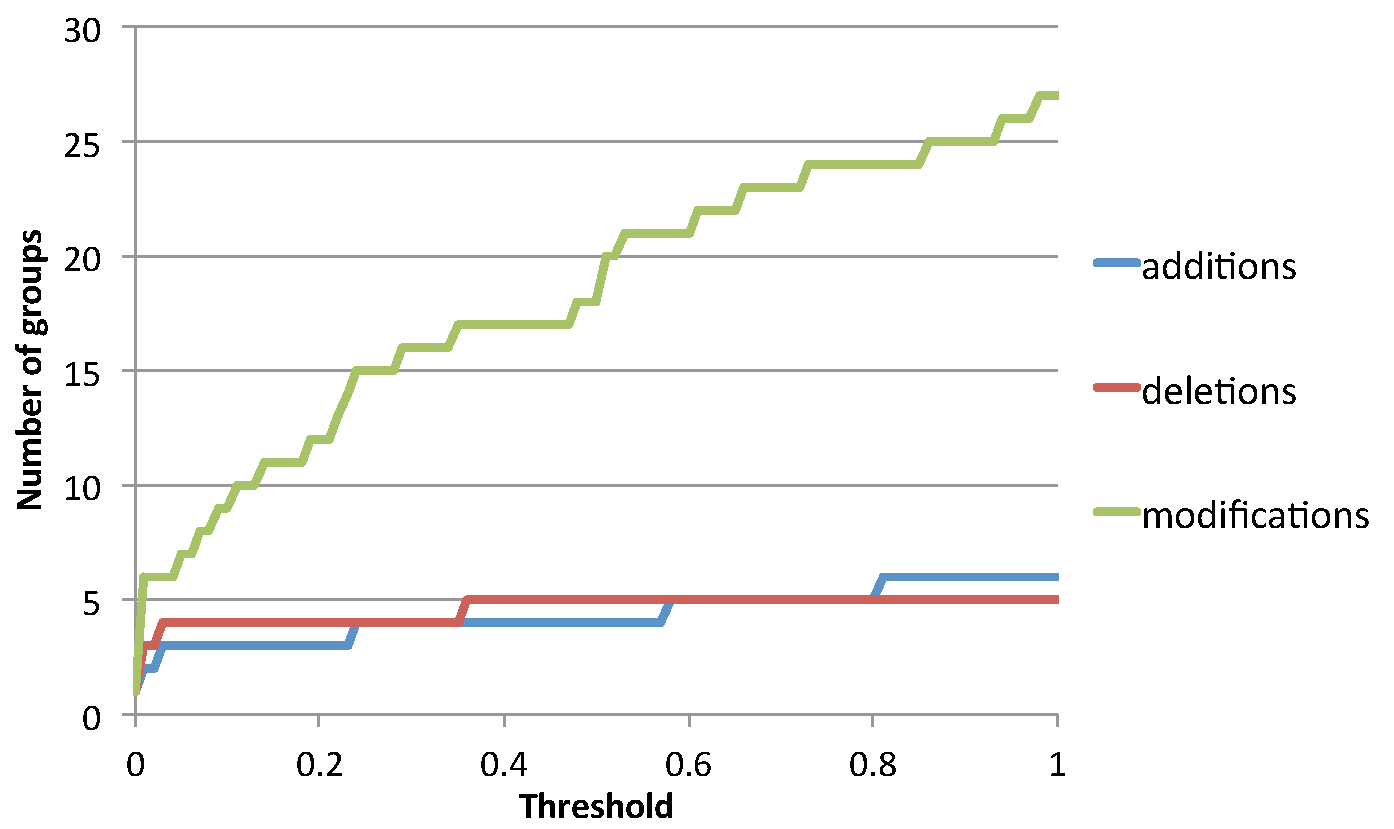
\includegraphics[width=\textwidth*0.2]{figures/clojure-number-of-modifications.pdf}
\end{figure}

\subsubsection{Removed code}
\begin{verbatim}
     for(int i=0;i < array.length;i+=2){
         init = f.invoke(init, array[i], array[i+1]);
-           if(RT.isReduced(init))
-                   return ((IDeref)init).deref();
         }
\end{verbatim}

\subsection{Interpretation of results}

